%!TEX root = /Users/carlos/Dropbox/Thesis/Thesis.tex
\section{Visualization} % (fold)
\label{sub:visualization}

The greatest challenge of this work was the creation of the visualization part for its requirements. We will now describe this part of Eagle Eye, its architecture, visualization techniques, sorting and filtering capabilities.

\subsection{Overview}
We wanted to make the visualization simple and easy to use, while keeping it flexible and capable enough to allow for an enjoyable and relevant experience.

After the backend has finished the all the processing that is needed, the visualization can be opened and all images that were added to the backend's processing list will appear in what we call the canvas. After loading the metadata, the user also presented with a set of options on the toolbar on the top, which is the only \ac{UI} needed to use the system (\fig{viz5141images}).

\begin{figure}[ht]
	\centering
		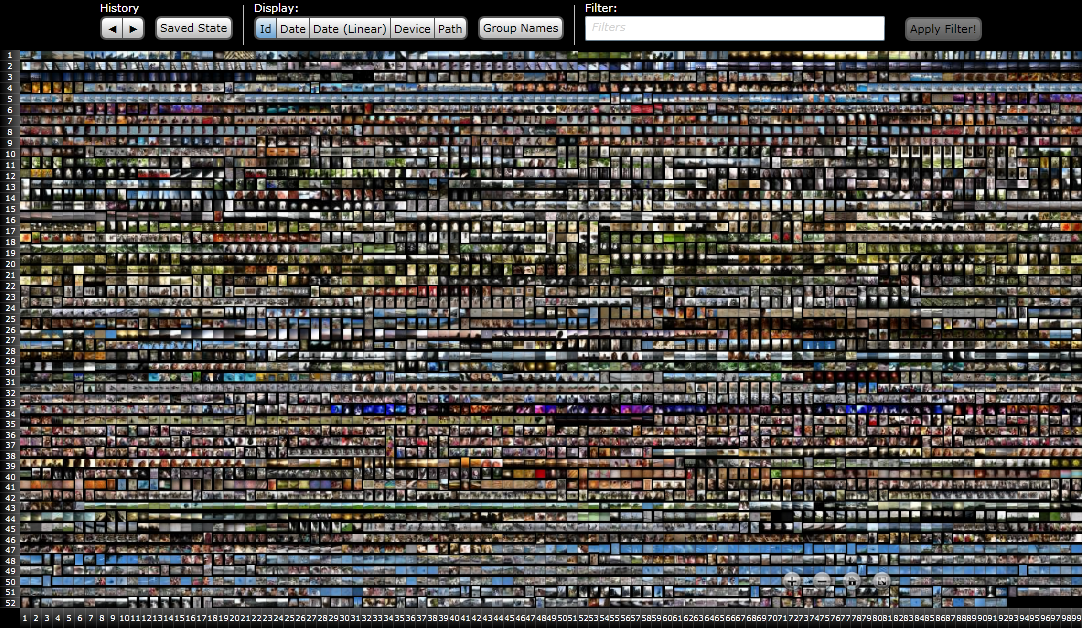
\includegraphics[width=\columnwidth]{Figures/viz5141images1082.png}
	\caption{Overview of the visualization. There are 5141 images are being displayed.}
	\label{fig:viz5141images}
\end{figure}

According to \todo{insert the reference of the dude who claimed that a 32x32px image was the minimum for recognition}, an image with 32 pixels per side is the minimum size that allows a user to recognize an image.

\red{Unsure about how well this fits here…} Upon loading Eagle Eye's visualization system, thousands of images might be displayed and this 32 pixel might not be met and, therefore, it might be difficult for the user to recognize what is on display from a single image, but since a lot of them are being displayed, the user might be capable of making sense of the groups by their main colors.

\subsubsection{The Canvas}

The canvas is the most relevant part of the visualization as it dynamically displays all the images previously selected by the user, at the same time. This may make the images barely recognizable and, therefore, the user has the possibility of manipulating the canvas to see and enjoy the images.
This means that the user can, at any time, use the mouse to drag the canvas around or, by clicking or scrolling, zoom in and out of the canvas. Zooming goes from the default view of thousands of images at the same time, until the full screen view of one of them, and everything in between in a smooth way.

\subsubsection{The toolbar}

\begin{figure}[htbp]
	\centering
		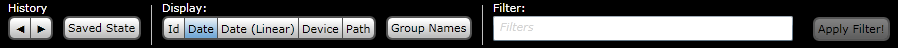
\includegraphics[width=\linewidth]{Figures/toolbar.png}
	\caption{The toolbar on top of the visualization \ac{UI}}
	\label{fig:toolbar}
\end{figure}


The user can then use the functions on the toolbar to filter and sort differently. The toolbar is divided in three sections: Navigation, Display and Filtering (\fig{toolbar}).

The navigation section contains some basic functions that work similarly to the current web browsers. There are buttons for back and forward between display states and a save button for bookmarking the current display state, allowing the user to easily get back to it later.

The middle section contains two options to change the image display: the sorting options and the display overlays button. The former presents the available sorting options for the current collection, based on the available metadata and on the best ways to display them. One of the options is selected at all times and the content is presented accordingly. Changing the selected option causes the images in display to move around to the new position and form a different sort order. This sorting and disposition options will be explained in a later section.
The other button in the display section of the toolbar enables or disables a layer of information on top of the images. This layer distinguishes the groups of images in display by painting them with a different colors and presents a name for them, depending on the selection sort option. Grouping will also be explained bellow. 

The third and final section of the toolbar is the filter section. It contains controls to filter images by using simple text and to visually select images on the canvas. This options will also be explained bellow.

\subsection{Disposition of Images on Canvas}
\label{sub:dispositions}

The different ways to dispose the images on the canvas was a matter that required some exploration of possibilities \refs. We chose a few options to allow some flexibility for the user, while trying to keep the interface simple.

We are now going to explain how do we sort images into groups and the different ways the user can arrange those groups on the canvas.

\subsubsection{Sorting images into groups}

As we've seen, the backend outputs metadata for each image. This metadata is loaded into the visualization application of Eagle Eye and is indexed by their type.

For instance, each image has an associated creation timestamp which will be aggregated by days, generating an image group for each day.

Similarly, the mean color associated with each image is indexed and groups are generated by dividing the hue spectrum in bins \todo{specify which and add the spectrum image}.

Another option is the grouping by device name, which usually allows to distinguish between who took the pictures if, for instance, different people have different cameras on the same event.

The last option currently available to the user is grouping by path which groups together the images that were already grouped by the user, on the file system. This allows for the display of an organization that is recognizable to the user, which can make a good starting point.

On the canvas, group boundaries are identifiable by discrete gray borders and, when the Show Overlays function is active, by color rectangles that also contain the groups' names.


\subsubsection{Different dispositions}

After having the images grouped by any of the sorting options referred on the previous section, the system has to know how to display them on the canvas.

We looked into various options \refs and picked the ones that we thought that made sense and also that would be easier for the user to understand. We chose a tree map view and a column-based linear view. Both of these are grid-based layouts, meaning that images are positioned inside a defined grid on the canvas. We also looked into free positioning systems like \refs but they make it harder for the user to understand the images within, since some images will be covered by others. When displaying thousands of images, it's important to make them easy to see, and mixing them up wasn't the appropriate thing to do. We focused on other ways for making it easier to the user see what matters and we will talk about them later on.

The first layout technique we employed was the tree map. The problem with tree maps is that they are designed for areas that can take many forms, from squares to thin lines \todo{insert tree map image}. Applying tree maps to images calls for the adaptation of the algorithms to make sure the areas can correctly hold the images and that all images in all groups have the same size and are positioned in the same grid, to make them easier to view. This ideas are supported by \todo{gajo} on his work in the Quantum treemaps. We tried to apply Quantum tree maps as our tree map algorithm but due to it's complexity and recurring problems, we adapted the tree maps of \todo{gajo}, as used in Prefuse \todo{verify} \refs to the reality of the image grid. This new algorithm was much easier to understand and implement, although  it might require a small fine running for a couple of edge cases.

Our tree map algorithm displays larger groups first, leaving the smaller ones to the end and makes an effort to layout groups as rectangles with an aspect ratio as close as possible to the screen's aspect ratio, for when the user zooms in, the groups fill the screen. There's also an effort to fill the space left between larger groups, making the display more compact and with less holes.

One problem of the tree map display is that group sequence is irrelevant. Groups are positioned by their size, which is unacceptable for sorting options that require some sequence, like sorting by time. For this we created a linear display that uses columns and displays groups sequentially. Each group may fill part of a column or various columns, depending on their size. With the aim of reducing wasted space, groups that fit on the wasted space left by the previous group use that space to display themselves. This is useful  to collapse the couple pictures the user might take of his regular day between days that he went on a trip and took a much larger number of photographs.

Currently we are using this layout system only for the date display since the use of columns makes visualization harder, requiring either some panning around the canvas or selecting the group using the filter tools explained ahead. This is an area we must improve, and we will discuss some ideas later on.


\subsubsection{Filtering} % (fold)

In addition to the sorting options explained above, Eagle Eye also provides the user with the ability to filter images. This allows the user to focus on a specific group of pictures that are his focus of interest at the moment.

For instance, the user might want to only see photos of a day, or a person, or person in a specific day or even pictures that are mostly blue.

For all this, Eagle Eye provides two ways to specify this kinds of constraints: using the filter bar or selecting pictures on the canvas, and we will now look into both them.

The filter bar's purpose mimics a regular search box, similar to the ones that exist on applications like Internet browsers, file browsers or photo browsers \refs: it provides a way for the user to type what he is looking for and get some suggestions to help him with the search. Since we wanted a simple \ac{UI}, we figured that we had to provide smart suggestions to the user, so that he can feel comfortable using it for multiple types of searches. Searches are performed immediately upon selecting the desired filter. Currently, searches are intersections (commonly ``and'') of the entries in the filter bar but after adding adequate \ac{UI}, it will be possible to also use unions (commonly ``or'').

Every piece of the metadata can be used as a filter and the suggestions list shows what are the available options and what type of metadata they relate to, for instance, when looking for a person's name, the ``keyword'' metadata type is shown, when searching for a place, both ``keyword'' and ``path'' types might be presented, if the path to the pictures included the place where they were taken.

This examples are quite simple but we wanted to go further and allow searches like ``Summer'', for all photos taken around the summer time in all years, ``May 2010'', for all pictures taken during that month, ``Has 2 people'' for photos that have been detected to have people in them. \red{Although some of these have not been implemented yet, they are in the plans.}

The second filter method allows the manual selection of images from the canvas, either by a common mouse drag-and-drop on the canvas or by selecting entire groups with a mouse click. This two interaction options can be activated on the respective button on the end of the toolbar \todo{image}. 

As explained above, the filter bar intersects its elements immediately after being added but that behavior in the function would make it impossible for the user to make multiple selections. So we made this feature allow various selections and only when the user forces the filtering that all the selections are unified and added to the rest of the intercession filters.

\red{Since the selections are displayed in the same way text filters are, the removal of a selection is made in the same way.}



\subsection{Architecture}

We will now take a look into the architecture of the visualization part of Eagle Eye.

\subsubsection{Metadata indexing}

At the center of the visualization is the DeepZoom canvas. By default, it displays images in the order they are specified on the ``collection.xml'' file, the file generated by the backend that identifies the multi-resolution imagery and images' metadata.

The ``collection.xml'' also contains some metadata for each image, added by the backend. The visualization parses the file and extracts this metadata which is then processed and indexed.

Since the transport is a text file, we used a simple, text based, key/value capable encoding \red{system}: JSON \refs. The backend encodes key/value pairs of metadata for each image \todo{meter um exemplo em código} and the visualization decodes and aggregates them in indexers, one indexer for each type of metadata. Eagle Eye has a few indexers that know how to read and process different types of data:
\begin{myitemize}
	\item{a generic indexer, for basic text or number values}
	\item{a date indexer, that gathers images by day}
	\item{a color indexer that gathers images by color, using \red{N} bins for \todo{lalala}}
	\item{a keyword indexer that indexes images by each one of the associated keywords}
	\item{a path indexer that indexes images by the folder where they resided when added}
\end{myitemize}

The indexers are managed by a metadata collection manager that handles, for instance, the XML parsing and creation and retrieval of indexers.

This indexers are the base for the sorting and disposition techniques we've covered on \ref{sub:dispositions}. Each indexer has attached the preferred way to be displayed, for instance, the path indexer works better when displayed using a tree map and thats what the ``Path'' button on the toolbar will use to dispose the images, but the date has two buttons, ``Date'' and ``Date (linear)'' because it makes sense for it to be displayed using both disposition techniques. \red{could be better}




\subsubsection{Canvas}

The canvas is the most important part of this work. Its core is from the DeepZoom framework and we use it to display lots of images in certain positions, according to the state of many variables. To hold all those options together and to help developing some more, we have created a state manager for the canvas.

A new canvas state object is created for each different set of options for the canvas. The object stores the options and computes the positioning of all images by picking those that have passed the filter, get the respective groups from the selected indexer, dispose them using the selected disposition algorithm and finally computing and saving the position for each image.

We use memoization to avoid repeated calculations for common display types. If a certain display has already been calculated, it will reuse the information on the saved state object to rearrange the canvas without going through the position calculations, allowing a faster interaction.


\subsubsection{Reducing Clutter}
\label{ss:stacks}

This work displays a great quantity of images at the same time and we thought that we could help the user by reducing some unnecessary clutter.

Sometimes users take more than one photo of the same thing and they do it for different reasons, some of them simple and others more technical. Some people just didn't like the previous photo or they want to make sure they have a few options to pick the best one and so they take more. Bursts of photographs are a similar case of this behavior but resulting in a larger image count.

Some more advanced photographic techniques require that the user takes more than one shot of something for merging in post processing. Examples of this techniques are panoramas, where a sequence of shots are merged to create a bigger image that what the camera lens is capable of, exposure bracketing, to overcome partial under or overexposure or focus bracketing, to increase the are of the image that is correctly focused.

Various shots of the same subject are generated by all of this motives and they clutter any image browser since they end up being multiple copies the same thing.

To help the user abstract himself from this similar images, we decided to come up with a way to collect them. Hsu et al. \cite{Hsu:2009p2696} used the idea of image grouping but probably not with a great implementation since it can be hard to see what is in the groups when they are collapsed and grouping was done manually. We chose a different path.

For our implementation, we decided to group images automatically based on the proximity of their capture timestamps, so every two images that were taken in a time span less then $t$ seconds are grouped together. After some experiments we decided on $t=4$ seconds which is more than enough for sequences of images that were taken automatically, gives some margin for manually taking another photo of the same thing, but is short enough for a regular user to take a picture, look at something else move the camera and take a picture of that.

For the display we decided to show all images of the group in the space of one, but displaying the first image at regular size and reducing the others to a smaller size, perceptible when looking closer and keeping the ability to zoom in on each of them and see them in fullscreen. This way we can reduce the clutter without fully hiding repeated images. \todo{images}

Obviously that this can have both false positives or false negatives but in our tests those were in a small number. \ac{UI} to fix that could be added but we don't feel that was essential.


%%%% Conclusion %%%%
\red{should make a section just for the chapter conclusion?}

To conclude this chapter, where we've seen what this work does and how it does it, we would like to add that many features and improvements could be added for an even better experience, but time and the focus of this work didn't allow us to do it. Even so, the Future Work (\ref{sec:futurework}) contains many ideas we have had which could bring this work to be a real world application.

% subsection visualization (end)

